\documentclass{ppjdoc}

\begin{document}

\title{Projektna dokumentacija}
\grupa{Grupa 15}
\datumpredaje{20.~siječnja 2010.}

\maketitle

\tableofcontents

\lstset{ %
basicstyle=\footnotesize \ttfamily,       % the size of the fonts that are used for the code
numbers=left,                   % where to put the line-numbers
numberstyle=\footnotesize,      % the size of the fonts that are used for the line-numbers
stepnumber=1,                   % the step between two line-numbers. If it's 1 each line will be numbered
numbersep=5pt,                  % how far the line-numbers are from the code
showspaces=false,               % show spaces adding particular underscores
showstringspaces=false,         % underline spaces within strings
showtabs=false,                 % show tabs within strings adding particular underscores
tabsize=3,	                % sets default tabsize to 2 spaces
captionpos=b,                   % sets the caption-position to bottom
breaklines=true,                % sets automatic line breaking
breakatwhitespace=false,        % sets if automatic breaks should only happen at whitespace
escapeinside={\%*}{*)}          % if you want to add a comment within your code
}

\chapter{Jezični procesori}

\section{Uvod}

Cilj jezičnog procesora je prevođenje višeg jezika, koji je razumljiv i ekspresivan, u niži jezik. Jezik kojeg prevodimo nazivamo izvorni jezik, a jezik u koji prevodimo nazivamo ciljni jezik. Jezični procesor je i sam program i jezik u kojem je napisan naziva se jezik izgradnje.

Kako bi se olakšala izgradnja jezičnog procesora njegov zadatak se rastavlja u više podzadataka koji slijede jedan iza drugoga: leksička analiza, sintaksna analiza, semantička analiza i sinteza (generiranje koda u ciljnom jeziku). Svaki od koraka ćemo ukratko opisati u uvodima drugih poglavlja.

\section{Naš jezični procesor}

Cilj nam je izgraditi jezični procesor koji prevodi izvorni jezik inspiriran C-om u ciljni jezik JVM \emph{bytecode}. Jezik izgradnje je programski jezik Java.

Ciljni jezik našeg jezičnog procesora je skoro pravi podskup programskog jezika C o kojem ne treba mnogo govoriti. 
U nastavku ćemo objasniti bitne razlike. Ciljni jezik je jezik koji razumije \emph{Java Vritual Machine}. Java je objektno-orijentirani jezik koje se također (slučajno) izvršava na JVM-u. Na JVM možemo gledati kao na sloj iznad same fizičke arhitekture računala pa to omogućava prenosivost programa.

Koristili smo pomoć nekih alata prilikom izrade leksičkog i sintaksnog analizatora. To su jFlex (generator leksičkog analizatora) i CUP (generator LR parsera).

\section{Neformalni opis izvornog jezika}

Kao što je rečeno, izvorni jezik je pojednostavljeni oblik programskog jezika C.

Tipovi podataka koje podržava su \texttt{int}, \texttt{float}, \texttt{char}, \texttt{boolean} i moguće je da 
funkcije ne vraćaju nikakav tip podataka tj. \texttt{void}. Deklariranje pokazivača nije moguće, no moguće je deklarirati
polja.

Za kontrolu toka se može koristiti petlje \texttt{for}, \texttt{while} i \texttt{do-while} i grananje \texttt{if-else}. 
I unutar petlji su mogući \texttt{break} i \texttt{continue}.
Ostalo nije podržano npr. \texttt{switch-case}, \texttt{goto}, \texttt{else if}.

Od operatora su podržani binarni: \texttt{<}  \texttt{>}  \texttt{==}  \texttt{<=}  \texttt{>=}  \texttt{!=}  \texttt{\&\&}  \texttt{||}  \texttt{!}  \texttt{+}  \texttt{-}  \texttt{*}  \texttt{/}  \texttt{\%}  \texttt{=}. Nije moguće koristiti \emph{bitwise} operatore. Od unarnih operator je podržan samo \texttt{-} i \texttt{!}. Nije moguće deklarirati više varijabli u jednom redu npr.
\texttt{int a, b, c;}. I nije moguće koristiti pretprocesorske naredbe (\texttt{include} i \texttt{define}).

Primjer ispravnog programa napisanog u izvornom jeziku:
\lstinputlisting[language=C]{primjer-uvod.c}



\chapter{Leksička analiza}

\section{Uvod}
Cilj leksičkog analizatora je grupirati znakove u smislene cjeline --- lekseme. Primjerice, identifikatore i ključne riječi.
Time ćemo olakšati rad sintaksnom analizatoru i izgradnju samog sintaksnog analizatora tj. gramatike.

Leksički analizator čita izvorni kôd znak po znak, grupira znakove u lekseme, odbacuje bjeline, prikuplja podatke koje može prikupiti u tom trenutku (vrsta leksema, tip konstante), pronalazi eventualne pogreške i određuje mjesto u programu gdje je došlo do nje.

Leksički analizatori se realiziraju pomoću konačnih automata, a praksa je da se pravila zadaju regularnim izrazima.

\section{Implementacija}

Za implementaciju smo koristili alat jFlex koji na temelju zadanih pravila generira leksički analizator. jFlex je
alat za progamski jezik Javu tj. kôd analizatora koji generira je u Javi.

Razred koji generira i koji predstavlja leksički analizator u našem se slučaju zove \texttt{Lexer}. Prilikom
instanciranja razreda \texttt{Lexer}, konstruktor prima \texttt{InputStream} iz kojeg čita ulaznu datoteku (izvorni kôd),
objekt razreda \texttt{Table} u koji će puniti informacije o leksemima (tip leksema, tip konstante) i listu u koju će
redom dodavati lekseme (kako bi ih kasnije mogli prikazati u tablici korisničkog sučelja).

Leksemi su predstavljeni razredom \texttt{Token} koji nasljeđuje razred \texttt{java\_cup.runtime.Symbol} (objekte tog razreda
očekuje sintaksni analizator generiran CUP-om, o tome kasnije). 

Razred \texttt{Lexer} ima metodu \texttt{next\_token()} koja vraća sljedeći leksem i nju prvenstveno koristi parser. Ukoliko
nije moguće vratiti leksem (zbog greške u kodu) onda se baca iznimka i prijavljuje se ta greška. 
No ispravljanje pogrešaka nije implementirano!

Rad sa \emph{stringovima} je zahtijevao korištenje razrješenja lijevog konteksta. To se ostvaruje s posebnim "leksičkim stanjem" u
koje leksički analizator uđe kad pročita \texttt{"} i dok je u njemu ignorira sva ostala leksička pravila. 

\section{Leksemi}

\section{Primjer izvođenja}

Primjer i prikaz izlaza našeg programa. Screenshot.


\chapter{Sintaksna analiza}

\section{Uvod}
Cilj sintaksne analize je provjeriti odgovara li niz leksema gramatičkoj strukturi (pravilima). Produkt
sintaksne analize (parsiranja) je sintaksno stablo. Gramatička pravila su zadana konteksno-neovisnom
gramatikom u BNF obliku.

Postoje razne tehnike parsiranja s raznim karakteristikama: skup jezika koji obuhvaćaju, težina
implementacije, pogodnost za automatsko generiranje parsera iz gramatike itd.

Naš sintaksni analizator gradi stablo tehnikom odozdo prema gore i spada u LR parsere. Tehnika
kojom generira tablicu prijelaza iz gramatike koju koristi parser se naziva LALR.

\section{Implementacija}

U implementaciji smo koristili generator LR parsera CUP koji generira parser napisan u programskom jezik Java.
Parser predstavlja razred \texttt{Parser} čiji konstruktor prima objekt razreda \texttt{Lexer}
kojeg koristi za dohvaćanje leksema.

Parser radi s objektima razreda \texttt{Symbol}. Oni mogu predstavljati završni (leksem) ili nezavršni znak gramatike.
Razred \texttt{Symbol} sadrži atribut \texttt{value} u koji pohranjujemo objekte razreda \texttt{TreeNode}. Razred
\texttt{TreeNode} predstavlja jedan čvor u sintaksnom stablu i čuva listu svoje djece.

U zadnjoj redukciji u nezavršni znak "program", atribut \texttt{value} će sadržavati vrh sintaksnog stabla i parser
će vratiti upravo taj vrh s kojim smo zapravo dobili cijelo stablo.

U CUP-u se osim produkcija zadaju i akcije koje se izvrše prilikom primjene redukcije određene produkcije. Upravo
te akcije koristimo za gradnju stabla pomoću \texttt{TreeNode}-ova.

\section{Gramatika}

Gramatika je dana u obliku kojeg prima CUP i može se vidjeti u dodatku A. Prednost operatora je rješenja pomoću CUP-a tako
da gramatika ostane što jednostavnija.

\section{Primjer izvođenja}
Pogledajmo primjer izvođenja sintaksne analize za sljedeći jednostavni program:

\lstinputlisting[language=C]{primjer-sintaksna1.c}

\begin{figure}[H]
  \centering
    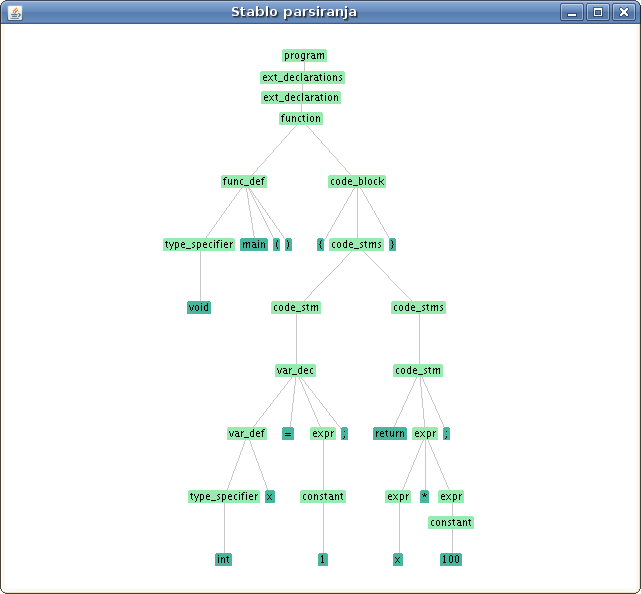
\includegraphics[width=13cm]{primjer-sintaksna1}
  \caption{Primjer izvođenja sintaksne analize}
\label{komponente}
\end{figure}


\chapter{Semantička analiza}

\section{Uvod}

Cilj semantičke analize je provjeriti i odrediti značenje pojedinih dijelova programa npr. provjeriti
je li varijabla koja se koristi deklarirana, odrediti tip podataka koji pripada nekom čvoru (npr. tipa \texttt{expr}
koji predstavlja aritmetičko-logički izraz).

Često se koristi sintaksnom vođena semantička analiza na način da se završni i nezavršni znakovi gramatike
prošire s atributima koji se izračunavaju prilikom parsiranja. CUP podržava takav način rada, no
mi ga nismo koristili. Naknadno, kad već dobijemo sintaksno stablo, obilazimo čvorove.

U našem jezičnom procesoru provjeravamo dvije osnovne stvari prilikom semantičke analize. Prva je da pazimo
na djelokruge varijabli i jesu li dostupne prilikom korištenja (jesu li uopće deklarirane). A druga je
da provjeravamo tipove podataka izraza. Informacije koje na taj način prikupimo prilikom semantičke
analize su nam iznimno bitne za generiranje ciljnog programa.


\section{Implementacija}
Semantički analizator je implementiran u razredu \texttt{SemanticAnalyzer}. Pozivom metode \texttt{analyze()}
pokreće se (ili nastavlja) analiza.

Prilikom analize obilazimo sintaksno stablo. Za to koristimo stog na koji stavljamo čvorove stabla.
U nekom koraku obilaska sa stoga skinemo jedan čvor, svu njegovu djecu stavimo na stog ali obrnutim redosljedom i 
obradimo skinuti čvor (često jednostavno nastavimo s obilaskom po stablu). To ponavljamo dok na stogu ima čvorova za obraditi. 
Na početku se na vrhu stoga nalazi vrh sintaksnog stabla.
Za određene tipove čvorova su definirane akcije koje se izvrše kada posjetimo te čvorove. 

Ukoliko posjetimo čvor tipa \texttt{expr} i za njega nije određen tip podataka onda rekurzivno 
odredimo tip. Na taj način se izvodi prvi dio semantičke analize. Drugi dio je malo kompliciraniji.

Izvorni jezik ima statički djelokrug bez ugnježđenja funkcija. 

Uz stog koji koristimo za obilazak, koristimo i stog na kojem čuvamo djelokruge. Djelokrug
je predstavljen razredom \texttt{Scope} i sastoji se u suštini od par hash-mapi koje čuvaju
popis varijabli koje su deklairane u tom djelokrugu, njihov tip i redni broj deklaracije (bitno za generiranje ciljnog programa).
Na vrhu tog stoga je uvijek trenutni aktivni djelokrug i sve deklaracije na koje naiđemo se odnose na njega.
Ukoliko se neka varijabla koristi u nekom izrazu onda provjerimo sve djelokruge (počevši od vrha stoga prema dnu)
sadrže li tu varijablu. Na početku je na vrhu stoga globalni djelokrug.

Ukoliko se dogodi da neka varijabla nije deklarirana, a pokuša se koristiti onda se prijavljuje greška. Semantička
analiza se nastavlja, no nakon nje, ukoliko postoje greške, ne pokreće se generiranje izlaznog koda.

\section{Primjer izvođenja i određivanja djelokruga}
Pogledajmo primjer određivanja djelokruga varijabli.

\lstinputlisting[language=C]{primjer-semanticka1.c}

\begin{figure}[H]
  \centering
    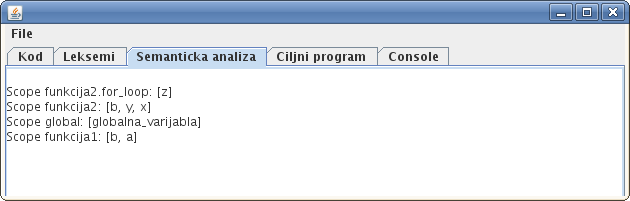
\includegraphics[width=13cm]{primjer-semanticka1}
  \caption{Primjer izvođenja semantičke analize}
\end{figure}

\pagebreak

Pogledajmo i jedan primjer gdje se koristi varijabla koja nije deklarirana (varijabla \texttt{z}).
\lstinputlisting[language=C]{primjer-semanticka2.c}

\begin{figure}[H]
  \centering
    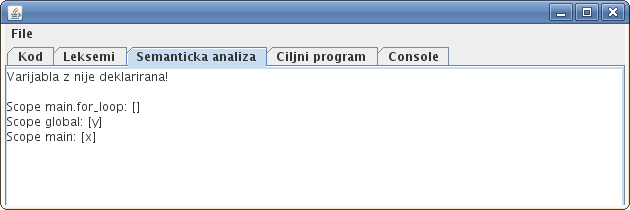
\includegraphics[width=13cm]{primjer-semanticka2}
  \caption{Primjer izvođenja semantičke analize s greškom u programu}
\label{komponente}
\end{figure}



\chapter{Generiranje ciljnog programa}

\section{Uvod}

U uvodu je rečeno da ciljni jezik JVM \emph{bytecode}. Java Virtual Machine (JVM) je virtualni stroj koji je prvenstveno
bio namijenjen programskom jeziku Java. Danas postoje razni jezici koji se prevode za JVM. Prednost je prenosivost
takvog koda.

JVM je stogovno orijentirane arhitekture tj. za izvođenje svih operacija se koristi stog. Također postoje 
registri iz kojih se mogu čitati i spremati podaci --- svakoj deklariranoj varijabli je dodijeljen jedan registar, a
indeks registra se određuje po redoslijedu deklariranja varijabli (unutar jedne funkcije tj. metode). 

Naš jezik nije objektno orijentiran jezik, a JVM je prvenstveno bio namijenjen objektno orijentiranoj Javi. Stoga
se svi naši izvorni programi prevode u razred \texttt{Program}, a deklarirane funkcije su zapravo javne metode
tog razreda. Evo primjera jednog programa napisanog u JVM \emph{bytecodeu}:

\lstinputlisting{primjer-bytecode.txt}

Vidimo da se radi o razredu \texttt{Program} koji nasljeđuje \texttt{Object} (takvo je pravilo u Javi)
i da taj razred ima jednu metodu \texttt{main} koja vraća \texttt{int} i ne prima nikakve argumente.

Naredba u liniji 4 stavlja na stog konstantu 10 i nakon toga (linija 5) vrh stoga (konstanta 10) sprema u registar 1.
To su naredbe \texttt{iconst} i \texttt{istore}, a prefix \texttt{i} označava da se radi o cjelobrojnom tipu podataka.

Linije 8 i 9 stave sadržaj registara 1 i 2 na stog. A u liniji 10 se poziva naredba \texttt{iadd} koja
s vrha stoga uzme dva elementa, zbroji ih, i rezultat pospremi na vrh stoga. Taj rezultat koji se sada
nalazi na vrhu stoga se s naredbom \texttt{istore} (linija 11) pospremi u registar 3.

Primjer izvornog koda koji bi se preveo u takav \emph{bytecode} je:

\lstinputlisting[language=C]{primjer-bytecode1.c}

Detaljne specifikacije o JVM bytecode je moguće naći u \cite{jvm}.

\section{Implementacija}

Generiranje nije u potpunosti implementirano. Dio koji je implementiran je implementiran unutar semantičke analize.

Implementirana je deklaracija varijabli i funkcija, obrada izraza (što uključuje i poziv funkcija), vraćanje vrijednosti i
\texttt{ if(expr) \{ ... \} } grananje za demonstraciju kontrole toka.

Kako je JVM stogovno orijentiran, a u sintaksnom stablu je pravilno očuvana prednost operatora, onda je
generiranje koda za izraze bilo jednostavno za ostvariti pomoću rekurzije. 

Također nije u potpunosti implementiran rad s tipovima podataka zbog nekih poteškoća i osobina JVM-a. Pa se u većini
slučajeva kao prefiks koji označava tip podataka koristi \texttt{i} tj. cjelobrojni tip.
\pagebreak
\section{Primjer izvođenja}

Pogledajmo prvo jednostavan primjer gdje su dani samo izrazi bez kontrole toka.

\lstinputlisting[language=C]{primjer-bytecode2.c}

\begin{figure}[H]
  \centering
    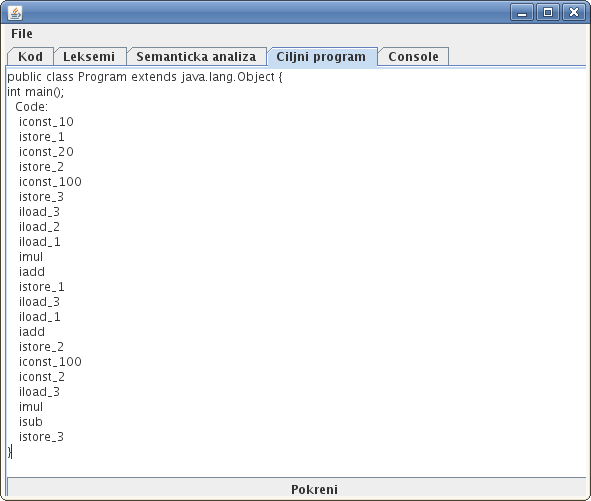
\includegraphics[width=13cm]{primjer-generiranje2}
  \caption{Primjer prevođenja jednostavnog programa}
\end{figure}

U drugom primjeru koristimo "if grananje" i poziv funkcije.

\lstinputlisting[language=C]{primjer-bytecode3.c}

\begin{figure}[H]
  \centering
    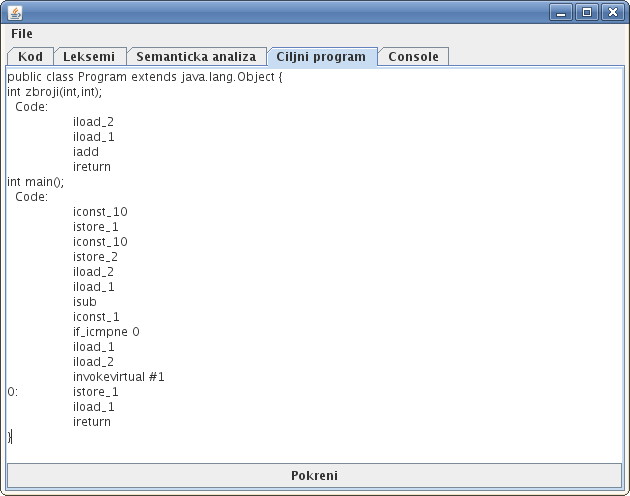
\includegraphics[width=13cm]{primjer-bytecode3}
  \caption{Primjer prevođenja}
\end{figure}



\chapter{Zaključak}

Prevođenje jezika nije jednostavan zadatak i kroz vrijeme su se razvile razne tehnike kojima se pokušava
olakšati taj proces. Tako se posao podijelio na podzadatke, no i svaki od njih je zahtjevan za implementirati.

Kod leksičke analize se regularni izrazi moraju prevesti u konačne automate, potrebno je minimizirati 
te automate i simulirati ih. Zbog toga su razvijeni generatori leksičkih analizatora poput jFlexa.

Sintaksnu analizu je još teže implementirati i zato su nastali alati poput CUP-a koji
iz zadane gramatike generiranju LALR metodom LR parser. LALR parseri su jedni od najraširenijih.

Problem sa semantičkom analizom je što ne postoji formalni način da se definiraju semantička 
pravila (za razliku od leksičke i sintaksne analize), no često se u praksi koristi
sintaksnom vođena semantička analiza koja može olakšati implementiranje semantičke analize.

Običaj je da se izvorni program prvo prevede u neki međukod koji je pogodan za optimiranje.
Mi nismo stigli implementirati korak optimiranja (koji je u praksi važan) zbog nedostatka
vremena pa naš prevoditelj direktno prevodi u ciljni jezik.


\pagebreak
\bibliography{literatura}

\appendix

\chapter{Gramatika}

\lstinputlisting{gramatika.txt} 


\end{document}
